\documentclass{article}
\usepackage[utf8]{inputenc}
\usepackage[russian]{babel}
\usepackage{amsfonts}
\usepackage{amsmath}
\usepackage{natbib}
\usepackage{upquote}
\usepackage{datetime}
\usepackage{multicol}
\usepackage{listings}
\usepackage{graphicx}

\setlength{\voffset}{-2cm}
\setlength{\textheight}{700pt}

\title{Численные методы: Домашняя работа}
\author{Группа 4001BV: Карина Пилюшонока}
\date \today

\begin{document}

\maketitle
\newpage
\tableofcontents
\newpage
\section{Расчет индивидуальных коэффициентов для заданий}
Номер группы: 4001BV \\
Номер в журнале: 16 \\
Год посутпления: 2010 \\
Форма обучения: вечерняя

\begin{displaymath} 
  N_{g} = 3 * (4 + 2) + 0 - 1 = 17
\end{displaymath}

\begin{displaymath}
  N_{s} = 16
\end{displaymath}
\section{Метод исключения Гаусса}
\subsection{Подготовка: расчет уравнений для индивидуального задания}
\begin{displaymath}
\left(
  \begin{array}{ccc}
    (N_{g}+4)+5i & -3-4i & 4-4i \\
    -3+2i & 8+(10-N_{s})i & 1+2i \\
    (N_{g}+1)i & N_{s}-10 & N_{s}-N_{g}i
  \end{array}
\right)
=
\left(
  \begin{array}{ccc}
    3+6i\\
    1-(N_{s}-20)i\\
    10i
  \end{array}
\right)
\end{displaymath}
После отброса мнимой части из уравнений получаем следующие коэффициенты для
уравнений:
\begin{displaymath}
\left(
  \begin{array}{ccc}
    21 x_{1} & -3 x_{2} & 4 x_{3} \\
    -3 x_{1} & 8 x_{2} & 1 x_{3} \\
    0 & 6 x_{2} & 16 x_{3}
  \end{array}
\right)
=
\left(
  \begin{array}{ccc}
    3\\
    1\\
    0
  \end{array}
\right)
\end{displaymath}

\subsection{Прямой ход Гаусса}
итерация: 1 

$I * -\frac{a_{21}}{a_{11}} + II$, где 
$I * -\frac{a_{21}}{a_{11}}$ принимает вид $3 - \frac{3}{7} + \frac{4}{7} =
\frac{3}{7}$
\begin{displaymath}
\left(
  \begin{array}{ccc}
    21 x_{1} & -3 x_{2} & 4 x_{3} \\
    0 & 7 \frac{4}{7} x_{2} & 1 \frac{4}{7} x_{3} \\
    0 & 6 x_{2} & 16 x_{3}
  \end{array}
\right)
=
\left(
  \begin{array}{ccc}
    3\\
    1\frac{3}{7}\\
    0
  \end{array}
\right)
\end{displaymath}
итерация: 2

$II * -\frac{a_{32}}{a_{22}} + III$, где 
$II * -\frac{a_{32}}{a_{22}}$ принимает вид $0 - 6 - 1\frac{13}{53} =
-1\frac{7}{53}$
\begin{displaymath}
\left(
  \begin{array}{ccc}
    21 x_{1} & -3 x_{2} & 4 x_{3} \\
    0 & 7 \frac{4}{7} x_{2} & 1 \frac{4}{7} x_{3} \\
    0 & 0 & 14\frac{40}{53} x_{3}
  \end{array}
\right)
=
\left(
  \begin{array}{ccc}
    3\\
    1\frac{3}{7}\\
    -1\frac{7}{53}
  \end{array}
\right)
\end{displaymath}

\subsection{Обратный ход Гаусса}

$x_{3} = -1\frac{7}{53} / 14\frac{40}{53} 
= -\frac{60}{53}/\frac{782}{53} 
= -\frac{60}{782} 
= -\frac{30}{391} \\$
$x_{2} = \frac{1\frac{3}{7} - 1\frac{4}{7} * (-\frac{30}{391})}{7 \frac{4}{7}} 
= (\frac{10}{7} + \frac{330}{2373}) / \frac{53}{7} 
= \frac{3910 + 330}{2737} / \frac{53}{7} 
= \frac{4240 * 7}{2737 * 53} 
= \frac{80}{391}\\$
$x_{1} = \frac{3 - 4*\frac{-30}{391} + 3*\frac{80}{391}}{21}
= (3 + \frac{120}{391} + \frac{240}{391})/21
= 3\frac{360}{391} / 21
= \frac{1533}{391 * 21} 
= \frac{73}{391}$
\begin{displaymath}
\mathbf{X} =
\left( \begin{array}{ccc}
  \frac{73}{391}\\ \\
  \frac{80}{391}\\ \\
  \frac{-30}{391} 
\end{array} \right)
\end{displaymath}

\subsection{Проверка}
yравнение 1:\\
$21 * \frac{73}{391} -3*\frac{80}{391} + 4 * \frac{-30}{391}
= \frac{1533}{391} - \frac{360}{391}
= \frac{1173}{391} 
= 3$
\\\\
yравнение 2:\\
$ -3 * \frac{73}{391} + 8*\frac{80}{391} + 1 *\frac{-30}{391}
= \frac{-219}{391} + \frac{640}{391} - \frac{-30}{391}
= 1$
\\\\
yравнение 3:\\
$0 + 6*\frac{80}{391} + 16 *\frac{-30}{391}
= \frac{480}{391} -\frac{480}{391} 
= 0$

\section{Методы приближения функции. Интерполяция и аппроксимация}

\subsection{Подготовка: расчет узлов}
\begin{table}[!h]
  \begin{tabular}{|l|l|l|l|l|}
  \hline
  \bfseries x & -1 & $N_{g}$   & 6 & 10\\
  \hline
  \bfseries y &  1 & $N_{s}-5$ & 8 & -2\\
  \hline
  \end{tabular}
\end{table}
При подстановке $N_{g}$ и $N_{s}$ получим следующий набор узлов:
\begin{table}[!h]
  \begin{tabular}{|l|l|l|l|l|}
  \hline
  \bfseries x & -1 & $17$ & 6 & 10\\
  \hline
  \bfseries y &  1 & $11$ & 8 & -2\\
  \hline
  \end{tabular}
\end{table}
 
\subsection{Полином Лагранжа}
Составляется полином для заданных узлов.
\begin{displaymath}
  \frac{(x-17)(x-6)(x-10)}{(-1-17)(-1-6)(-1-10)} *1 +
  \frac{(x+1)(x-6)(x-10)}{(17+1)(17-6)(17-10)} * 11 + \\
  \frac{(x+1)(x-17)(x-10)}{(6+1)(6-17)(6-10)} * 8 + 
  \frac{(x+1)(x-17)(x-6)}{(10+1)(10-17)(10-6)} * (-2)
\end{displaymath}

Далее, раскрываются скобки, а также в 1ой и 4ой дроби меняем знак изза
полученных знаков в знаменателе.
\begin{displaymath} 
  \frac{-x^3 + 33x^2 - 332x + 1020}{1386} +
  \frac{11x^3 - 165x^2 + 484x + 660}{1386} + 
  \frac{8x^3 -208x^2 + 1144x + 1360}{308} + 
  \frac{2x^3 - 44x^2 + 158x + 204}{308}
\end{displaymath}

Далее складываем попарно дроби (1+2 и 3+4).
\begin{displaymath} 
  \frac{-x^3 + 33x^2 - 332x + 1020 + 11x^3 - 165x^2 + 484x + 660}{1386} +
  \frac{8x^3 -208x^2 + 1144x + 1360 + 2x^3 - 44x^2 + 158x + 204}{308} = \\
  \frac{10x^3 + -132x^2 + 152x + 1680 }{1386} +
  \frac{10x^3 -252x^2 + 1302x + 1564}{308} = \\
  \frac{10x^3 + -132x^2 + 152x + 1680 }{1386} +
  \frac{5x^3 -126x^2 + 651x + 782}{154}    
\end{displaymath}

Приведение дроби к общему знаменателю. Для 1386 и 154 НОК является 1386 
($1386 * 1 = 1386$ и $154 * 9 = 1386$).

\begin{displaymath} 
  \frac{10x^3 + -132x^2 + 152x + 1680 }{1386} -
  \frac{5x^3 -126x^2 + 651x + 782}{154} = 
  \frac{10x^3 + -132x^2 + 152x + 1680 + 45x^3 - 1134x^2 + 5859x + 7038}{1386}=
  \frac{55x^3 - 1266x^2 + 6011x + 8718}{1386}
\end{displaymath}

\subsection{Полином Ньютона}
Порядок вычислений коэффициентов для полинома.
\begin{table}[!h]
  \begin{tabular}{|l|l|l|l|l|l|}
  \hline
  \bfseries \#& x  & y0  & y1 & y2 & y3\\
  \hline
  \bfseries 1 & -1 & 1  &    &    &  \\  
  \hline
  \bfseries   &    &    & $\frac{11-1}{17+1} = \frac{5}{9}$ &  & \\  
  \hline
  \bfseries 2 & 17 & 11 & & $\frac{\frac{3}{11} - \frac{5}{9}}{6+1} =
   \frac{27 - 55}{99 * 7} =
   \frac{-4}{99}$ & \\
  \hline
  \bfseries   &    &    & $\frac{8-11}{6-17} = \frac{3}{11}$ & 
  & $\frac{\frac{61}{154} + \frac{4}{99}}{10+1} =
  \frac{549 + 56}{1386 * 11} = 
  \frac{5}{126}$\\
  \hline
  \bfseries 3 & 6  & 8  & & $\frac{\frac{-5}{2} - \frac{3}{11}}{10-17} =
  \frac{-55 - 6}{22 * (-7)} =
  \frac{61}{154}$ & \\
  \hline
  \bfseries   &    &    & $\frac{-2-8}{10-6} = \frac{-5}{2}$ & & \\
  \hline
  \bfseries 4 & 10 & -2 & & & \\
  \hline
  \end{tabular}
\end{table} 

Используя значения таблицы, составим интерполирующий полином.
\begin{displaymath} 
  N(x) = y0_1 + y1_{1} *(x-x_1) + y2_1 *(x-x_1)*(x-x_2) +
  y3_1*(x-x_1)*(x-x_2)*(x-x_3) 
\end{displaymath}
\begin{displaymath} 
  N(x) = 1 + \frac{5}{9}(x+1) - \frac{4}{99}(x+1)(x-17) +
  \frac{5}{126}(x+1)(x-17)(x-6)
\end{displaymath}


\subsection{Метод наименьших квадратов}
$\phi_k(x) = a_0 + a_1x + a_2x + \ldots + a_kx^k$
Рассмотрим 3 варианта МНК:
\begin{itemize}
  \item аппроксимация, при порядке $n-2 = 2$;
  \item интерполяция, при порядке $n-1 = 3$;
  \item при порядке $n$.
\end{itemize}

\subsubsection{k=2}
$\phi_k(x) = a_0 + a_1x + a_2x^2$\\
Составим систему:
\begin{displaymath}
\left(
  \begin{array}{ccc}
    4 a_{0} & 32 a_{1} & 426 a_{2} \\
    32 a_{0} & 426 a_{1} & 6128 a_{2} \\
    426 a_{0} & 6128 a_{1} & 94818 a_{2} 
  \end{array}
\right)
=
\left(
  \begin{array}{ccc}
    18\\
    214\\
    3268
  \end{array}
\right)
\end{displaymath}
Используя метод решения систем ЛУ Гаусса, получим результат метода МНК при
степени 2 (аппроксимация):
\begin{displaymath}
\phi_k(x) = 
  2.0435446906035106 -
  0.21161191749426933 \cdot x +
  0.038961038961038905 \cdot x^2
\end{displaymath}

\subsubsection{k=3}
$\phi_k(x) = a_0 + a_1x + a_2x + a_3x^3$\\
Составим систему:
\begin{displaymath}
\left(
  \begin{array}{cccc}
    4 a_{0} & 32 a_{1} & 426 a_{2} & 6128 a_{3}\\
    32 a_{0} & 426 a_{1} & 6128 a_{2} & 94818 a_{3}\\
    426 a_{0} & 6128 a_{1} & 94818 a_{2} & 1527632 a_{3} \\
    6128 a_{0} & 94818 a_{1} & 1527632 a_{2} & 25184226 a_{3} 
  \end{array}
\right)
=
\left(
  \begin{array}{ccc}
    18\\
    214\\
    3268\\
    53770
  \end{array}
\right)
\end{displaymath}
Используя метод решения систем ЛУ Гаусса, получим результат метода МНК при
степени 3 (предельный случай - интеполяция):\\
$ \phi_k(x) = 
  6.290043290043431 +
  4.336940836941042 \cdot x -
  0.9134199134199545 \cdot x^2 +
  0.03968253968254137 \cdot x^3
$
\subsubsection{k=4}
$\phi_k(x) = a_0 + a_1x + a_2x + a_3x^3 + a_4x^4$\\
Составим систему:
\begin{displaymath}
\left(
  \begin{array}{ccccc}
    4 a_{0} & 32 a_{1} & 426 a_{2} & 6128 a_{3} & 94818 a_{4}\\
    32 a_{0} & 426 a_{1} & 6128 a_{2} & 94818 a_{3} & 1527632_{4}\\
    426 a_{0} & 6128 a_{1} & 94818 a_{2} & 1527632 a_{3} & 25184226 a_{4}\\
    6128 a_{0} & 94818 a_{1} & 1527632 a_{2} & 25184226 a_{3} & 420618608 a_{4}\\
    94818 a_{0} & 1527632 a_{1} & 25184226 a_{2} & 420618608 a_{3} & 7077437058 a_{4}\\
  \end{array}
\right)
=
\left(
  \begin{array}{ccc}
    18\\
    214\\
    3268\\
    53770\\
    909100
  \end{array}
\right)
\end{displaymath}
Используя метод решения систем ЛУ Гаусса, получим результат метода МНК при
степени 4: \\
$ \phi_k(x) =
  5.298582534229462 +
  3.6681908369409446 \cdot x -
  0.6227858291176097 \cdot x^2 + 
  0.008577888519749872 \cdot x^3 + 
  0.0009720203488372093 \cdot x^4
$

\subsection{Графическое отображение}

\section{Методы численного интегрирования и дифференцирования}
\subsection{Метод прямоугольников}
\subsection{Метод трапеций}
\subsection{Метод Симпсона}
\subsection{Квадратура Гаусса}

\section{Решение нелинейного уравнения}
\subsection{Подготовка: создание уравнения, вспомогательные элементы}

\begin{displaymath}
  \begin{array}{ccc}
    f(x) = x / sin^2(3x)  \\
    f'(x) = (1 - 6x cos(3 x) / sin(3 x)) 1/sin^2(3 x)\\
    f''(x) = 6/sin^4(3x) * (6x - sin(6x) + 3x * cos(6x))
  \end{array}
\end{displaymath}

\begin{displaymath}
  \begin{array}{ccc}
    f(x) = N_{g}  \\
    x / sin^2(3x) = 17 \\
    x / sin^2(3x) - 17 = 0 \\
  \end{array}
\end{displaymath}

Точность: $\varepsilon = 0.0001$

Интервал для поиска корней: [0.1; 1]

\subsection{Метод бисекции}
Итерация: 1 \\
\begin{math}
  x_{0}= (0.1+1)/2 = 0.55\\
  a=0.1, b=1\\
  b-a > \varepsilon \\
  f(a) = 1.14505, f(x) = 0.553465\\
  f(a) * f(x) > 0\\
  a = 0.55
\end{math}\\\\
итерация: 2\\
\begin{math}
  x_{1}= (0.55+1)/2 = 0.775\\
  a=0.55, b=1\\
  b-a > \varepsilon \\
  f(a) = 0.553465, f(x) = 1.45903\\
  f(a) * f(x) > 0\\
  a = 0.775
\end{math}\\\\
итерация: 3\\
\begin{math}
  x_{2}= (0.775+1)/2 = 0.8875\\
  a=0.775, b=1\\
  b-a > \varepsilon \\
  f(a) = 1.45903, f(x) = 4.17653\\
  f(a) * f(x) > 0\\
  a = 0.8875
\end{math}
итерация: 4
\begin{math}
  x_{3}= (0.8875+1)/2 = 0.94375\\
  a=0.8875, b=1\\
  b-a > \varepsilon \\
  f(a) = 4.17653, f(x) = 10.1196\\
  f(a) * f(x) > 0\\
  a = 0.94375
\end{math}\\\\
итерация: 5\\
..закончила тут
\begin{math}
  x_{4}= (0.8875+1)/2 = 0.94375\\
  a=0.8875, b=1\\
  b-a > \varepsilon \\
  f(a) = 4.17653, f(x) = 10.1196\\
  f(a) * f(x) > 0\\
  a = 0.94375
\end{math}\\\\

\begin{displaymath}
  x: 0.971875, ab = [0.94375, 1];
\end{displaymath}
итерация: 6
\begin{displaymath}
  x: 0.9578125, ab = [0.94375, 0.971875].
\end{displaymath}

Результат: $x = 0.966876220703125$, за 14 итераций.

\subsection{Метод хорд}
Условие сходимости метода: 
\begin{displaymath}
  \begin{array}{ccc}
    f(1) = x / sin^2(3x) = 33.213768360408736 \\
    f''(1) = 6/sin^4(3x) * (6x - sin(6x) + 3x * cos(6x)) = 138576.26831776567
  \end{array}
\end{displaymath}
- знак не меняется, значит метод применим.\\
Итерация: 1
\begin{displaymath} 
  x: 0.3908054983496253, ab = [0.1, 1]
\end{displaymath}
итерация: 2
\begin{displaymath}
  x: 0.5933240899277314, ab = [0.3908054983496253, 1]
\end{displaymath}
итерация: 3
\begin{displaymath}
  x: 0.7276420688960742, ab = [0.5933240899277314, 1]
\end{displaymath}
итерация: 4
\begin{displaymath}
  x: 0.8158659960100441, ab = [0.7276420688960742, 1]
\end{displaymath}
итерация: 5
\begin{displaymath}
  x: 0.8731678144064535, ab = [0.8158659960100441, 1]
\end{displaymath}
итерация: 6
\begin{displaymath}
  x: 0.9098002888447452, ab = [0.8731678144064535, 1]
\end{displaymath}

Результат: $x = 0.9668512818566148$, за 18 шагов.

\subsection{Метод Ньютона}
\begin{displaymath}
  x_{0}: 0.55;
\end{displaymath}
Итерация: 1
\begin{displaymath}
  x: 13.50135782145894  delta: 12.95135782145894;
\end{displaymath}
итерация: 2
\begin{displaymath}
  x: 13.451261598353025  delta: 0.05009622310591588;
\end{displaymath}
итерация: 3
\begin{displaymath}
  x: 13.387853446812523  delta: 0.06340815154050183;
\end{displaymath}
итерация: 4
\begin{displaymath}
  x: 13.321324383604663  delta: 0.06652906320785945;
\end{displaymath}
итерация: 5
\begin{displaymath}
  x: 13.272783216385665  delta: 0.04854116721899793;
\end{displaymath}
итерация: 6
\begin{displaymath}
  x: 13.254786613462766  delta: 0.017996602922899285.
\end{displaymath}

Результат: $x = 13.252873093705627$, за 8 итераций.
\subsubsection{Метод Ньютона: пояснение результата}
  Метод Ньютона, при начальном $x_{0} = 0.55$ не сходится (см.
  Рис.\ref{equ_newton_img}).
  \begin{figure}[b]
    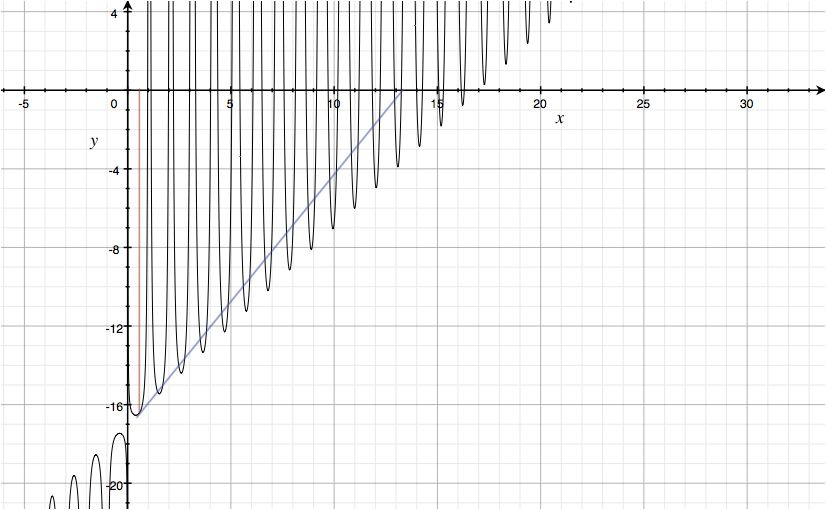
\includegraphics[width=13cm]{equations_newton.png}
    \caption{Первые шаги поиска корня методом Ньютона для функции $x/sin^2(3x)
    - 17$}
    \label{equ_newton_img}
  \end{figure}

\subsection{Метод простых итераций}

\section{Решение линейного дифференциального уравнения 2-го порядка}
\subsection{Метод Рунге-Кутта}

\section{Разложение периодической функции в ряд Фурье}

\end{document}
